%%%%%%%%%%%%%%%%%%%%%%%%%%%%%%%%%%%%%%%%%
% Beamer Presentation
% LaTeX Template
% Version 1.0 (10/11/12)
%
% This template has been downloaded from:
% http://www.LaTeXTemplates.com
%
% License:
% CC BY-NC-SA 3.0 (http://creativecommons.org/licenses/by-nc-sa/3.0/)
%
%%%%%%%%%%%%%%%%%%%%%%%%%%%%%%%%%%%%%%%%%

%------------------------------------------------------------------------------------------------
% PACKAGES AND THEMES
%------------------------------------------------------------------------------------------------

\documentclass[table, xcolor = {dvipsnames}, 9pt]{beamer}
\usepackage{tikz}
\usetikzlibrary{calc}
\usetikzlibrary{positioning}
\usetikzlibrary{arrows.meta}
\usetikzlibrary{external}
\mode<presentation> {

% The Beamer class comes with a number of default slide themes
% which change the colors and layouts of slides. Below this is a list
% of all the themes, uncomment each in turn to see what they look like.

\usetheme{default}
%\usetheme{AnnArbor}
%\usetheme{Antibes}
%\usetheme{Bergen}
%\usetheme{Berkeley}
%\usetheme{Berlin}
%\usetheme{Boadilla}
%\usetheme{CambridgeUS}
%\usetheme{Copenhagen}
%\usetheme{Darmstadt}
%\usetheme{Dresden}
%\usetheme{Frankfurt}
%\usetheme{Goettingen}
%\usetheme{Hannover}
%\usetheme{Ilmenau}
%\usetheme{JuanLesPins}
%\usetheme{Luebeck}
%\usetheme{Madrid}
\usetheme{metropolis}
%\usetheme{Malmoe}
%\usetheme{Marburg}
%\usetheme{Montpellier}
%\usetheme{PaloAlto}
%\usetheme{Pittsburgh}
%\usetheme{Rochester}
%\usetheme{Singapore}
%\usetheme{Szeged}
%\usetheme{Warsaw}

% As well as themes, the Beamer class has a number of color themes
% for any slide theme. Uncomment each of these in turn to see how it
% changes the colors of your current slide theme.

%\usecolortheme{albatross}
%\usecolortheme{beaver}
%\usecolortheme{beetle}
%\usecolortheme{crane}
%\usecolortheme{dolphin}
%\usecolortheme{dove}
%\usecolortheme{fly}
%\usecolortheme{lily}
%\usecolortheme{orchid}
%\usecolortheme{rose}
\usecolortheme{seagull}
%\usecolortheme{seahorse}
%\usecolortheme{whale}
%\usecolortheme{wolverine}
\usefonttheme{professionalfonts}
%\setbeamertemplate{footline} % To remove the footer line in all slides uncomment this line
%\setbeamertemplate{footline}[page number] % To replace the footer line in all slides with a simple slide count uncomment this line

%\setbeamertemplate{navigation symbols}{} % To remove the navigation symbols from the bottom of all slides uncomment this line
}

\usepackage{graphicx} % Allows including images
\usepackage{booktabs} % Allows the use of \toprule, \midrule and \bottomrule in tables
\usepackage{tikz}
\usepackage{multirow}
\usepackage{natbib}
\usepackage{hyperref}
\usepackage{diagbox}
\usepackage{makecell}
\usepackage{xparse}
\usepackage{subfig}
\usepackage{amsmath}
\usepackage{amsfonts,amsthm,amsmath,amssymb}    
\usepackage{bbm}
\usepackage{bm}
\usepackage{empheq}
\usepackage{pgfplots}
\usepackage{animate}
\usepgfplotslibrary{colorbrewer}

\newcommand\mybox[2][]{\tikz[overlay]\node[fill=lightgray,inner sep=2pt, anchor=text, rectangle, rounded corners=1mm,#1] {#2};\phantom{#2}}
\hypersetup{unicode=true,
            bookmarksnumbered=true,
            bookmarksopen=true,
            bookmarksopenlevel=2,
            breaklinks=false,
            pdfborder={0 0 1},
            hypertexnames=false,
            pdfstartview={XYZ null null 1}}
\usepackage{xcolor}
\newcommand\myheading[1]{%
  \par\bigskip
  {\Large\bfseries#1}\par\smallskip}
\newcommand\given[1][]{\:#1\vert\:}
\theoremstyle{plain}
\newtheorem{thm}{Theorem}
\newtheorem{prop}{Proposition\thisthmnumber}
\newtheorem{lem}{Lemma\thisthmnumber}
\newtheorem{cor}{Corollary}
\newtheorem{defin}{Definition}
\newtheorem{algo}{Algorithm}
\newcommand*\diff{\mathop{}\!\mathrm{d}}
\newcommand*\Diff[1]{\mathop{}\!\mathrm{d^#1}}
\newcommand{\bh}[1]{{\color{blue}{#1}}}
\newcommand{\mh}[1]{{\color{magenta}{#1}}}
\newcommand{\thisthmnumber}{}
\newcommand{\tikzmark}[1]{\tikz[baseline,remember picture] \coordinate (#1) {};}
\newcommand*{\QEDA}{\hfill\ensuremath{\blacksquare}}%
\newcommand*{\QEDB}{\hfill\ensuremath{\square}}%
\DeclareMathOperator{\E}{\rm{E}}
\DeclareMathOperator{\R}{\mathbb{R}}
\DeclareMathOperator{\N}{\mathbb{N}}
\DeclareMathOperator{\Var}{\rm{Var}}
\DeclareMathOperator{\Cov}{\rm{Cov}}
\DeclareMathOperator{\Supp}{\rm{Supp}}
\DeclareMathOperator{\e}{\rm{e}}
\DeclareMathOperator{\F}{\mathcal{F}}
\DeclareMathOperator{\Z}{\mathcal{Z}}
\DeclareMathOperator{\logit}{\rm{logit}}
\DeclareMathOperator{\indep}{{\perp\!\!\!\perp}}
\DeclareMathOperator{\rank}{rank}
\DeclareMathOperator*{\argmin}{arg\,min}
\DeclareMathOperator*{\argmax}{arg\,max}
%\DeclareMathOperator{\Pr}{\rm{Pr}}
%------------------------------------------------------------------------
% TITLE PAGE
%-----------------------------------------------------------------------
\pagestyle{empty}
\title[]{Estimation of Average Causal Effects} % The short title appears at the bottom of every slide, the full title is only on the title page

\author{Thomas Leavitt} % Your name
\institute[] % Your institution as it will appear on the bottom of every slide, may be shorthand to save space
{
% Your institution for the title page
\medskip
\textit{} % Your email address
}
\date{\today} % Date, can be changed to a custom date

\begin{document}

\begin{frame}
\titlepage % Print the title page as the first slide
\end{frame}

%\begin{frame}
%\frametitle{Overview} % Table of contents slide, comment this block out to remove it
%\tableofcontents % Throughout your presentation, if you choose to use \section{} and \subsection{} commands, these will automatically be printed on this slide as an overview of your presentation
%\end{frame}

%------------------------------------------------------------------------
% PRESENTATION SLIDES
%------------------------------------------------------------------------
\section{Potential Outcomes Framework}

\begin{frame}{Causality with Potential Outcomes}
  \begin{itemize}
  \item Definition: \bh{Treatment}
  \item[] $Z_i$: Indicator of treatment assignment for {\em unit} $i$, where $i = 1, \ldots, N$
    \[
      Z_i = \left\{
        \begin{array}{ll}
          1 & \mbox{if unit $i$ receives treatment}\\
          0 & \mbox{otherwise}
        \end{array}
      \right.
    \]
\pause
  \item Definition: \bh{Potential Outcomes}
  \item[] \indent $y_{Ti}$ or $y_{Ci}$: Fixed value of the outcome for unit $i$ if it were to receive treatment or control
  \item[] E.g., $y_{Ti}$: voter turnout of person $i$ if person $i$ were to receive mail encouraging turnout
  \item[] E.g., $y_{Ci}$: voter turnout of person $i$ if person $i$ were \textit{not} to receive mail encouraging turnout
  \end{itemize}
\end{frame}
%------------------------------------------------------------------------
\begin{frame}{Defining Causal Effects + Observed Outcomes}
\begin{itemize}
\item Causal effect (treatment effect) for unit $i$
\item[] \mh{Additive} causal effect of the treatment on the outcome for unit $i$:
\begin{eqnarray*}
\tau_i & = & y_{Ti} - y_{Ci}
\end{eqnarray*}
\item Other functions of of individual potential outcomes possible, e.g., $\dfrac{y_{Ti}}{y_{Ci}}$ \pause
\item \mh{Fundamental Problem of Causal Inference} (Holland 1986):
  \begin{center}
    We can never observe both $y_{Ti}$ and $y_{Ci}$ for the same $i$\\
  \end{center} 
\item We can observe only one of the two potential outcomes:
  $$ Y_i = Z_i y_{Ti} + (1 - Z_i)y_{Ci}$$
\item Therefore, $\tau_{i}$ is unobserved for every unit
\end{itemize}
\end{frame}
%------------------------------------------------------------------------
\section{The average treatment effect}
\begin{frame}
\frametitle{Average treatment effect: An example} 
\begin{itemize}
\item Definition: \bh{Average Treatment Effect (ATE)}
\begin{eqnarray*}
\tau & = &  \frac{1}{N}\sum_{i = 1}^N \left(y_{Ti} - y_{Ci} \right)
\end{eqnarray*} \pause
\item Example: \bh{``Village heads'' study} (Gerber and Green 2012, Chapter 2): \vspace{0.1in}
\item[]
\begin{center}
\begin{tabular}{l|rrr} \hline
& \multicolumn{3}{c}{Budget share (\%)} \\
Village &$\bm{y_C}$& $\bm{y_T}$& $\bm{\tau}$  \\ \hline
1& 10 & 15  & 5  \\
2& 15 & 15  & 0   \\ 
3& 20 & 30  & 10   \\
4& 20 & 15  & -5   \\
5& 10 & 20  & 10   \\
6& 15 & 15  & 0   \\
7& 15 & 30  & 15   \\ \hline
Average & 15 & 20 & 5  \\ \hline
\end{tabular}
\end{center}
\end{itemize}
\end{frame}
%------------------------------------------------------------------------
\section{Randomized experiments}
\begin{frame}
  \frametitle{Basic Setup for Randomized Experiment}
  \begin{itemize}
  \item Units: $i = 1, \ldots, N $
  \item Treatment: $Z_i = 0$ or $Z_i = 1$ is randomly assigned     
  \item Potential outcomes: $y_{Ci}$ and $y_{Ti}$
  \item Observed outcome: $Y_i = Z_i y_{Ti} + (1 - Z_i) y_{Ci}$
    \vspace{0.1in} \pause
  \item Treatment Assignment Mechanism
  \item[] (1) \mh{Bernoulli (simple) randomization}: Each unit is
    independently assigned to treatment with probability $p$
  \item[] (2) \mh{Complete randomization}: Exactly $n_T$ units are treated and $N - n_T = n_C$ units are untreated
  \item[] (3) In practice, (1) and (2) are equivalent when we fix $n_T$ by conditioning on its observed value
    \vspace{0.1in}
  \item Under complete or simple (conditioning on observed $n_T$) randomization
$$
\E\left[Z_i\right] = \dfrac{n_T}{N}
$$
  \end{itemize}
\end{frame}
%------------------------------------------------------------------------
\section{Difference-in-Means estimator}
\begin{frame}
  \frametitle{Unbiasedness of Difference-in-Means: Proof}
  \small
  \begin{itemize}
  \item \mh{Difference-in-Means estimator}
    \begin{align*}
      \hat{\tau}\left(\bm{Z}, \bm{Y}\right) & = n_T^{-1} \bm{Z}^{\top} \bm{Y} - n_C^{-1} \left(\bm{1} - \bm{Z}\right)^{\top}\bm{Y} \\ 
      & = \frac{1}{n_T} \sum_{i=1}^N Z_i Y_i - \frac{1}{n_C} \sum_{i = 1}^N (1 - Z_i) Y_i
    \end{align*} \pause
  \item \mh{Unbiased} for the ATE under complete randomization \pause
  \item[] 
    {\footnotesize
      \begin{eqnarray*}
        \hspace{-0.4in} \E\left[\hat{\tau}\left(\bm{Z}, \bm{Y}\right)\right] & = & \E\left[\frac{1}{n_T} \sum_{i=1}^N Z_i Y_i - \frac{1}{n_C} \sum_{i = 1}^N (1 - Z_i) Y_i\right]\\
        \hspace{-0.4in} & = &  \frac{1}{n_T} \sum_{i=1}^N \E\left[Z_i Y_i\right]
                              - \frac{1}{n_C} \sum_{i=1}^N \E\left[(1 - Z_i) Y_i\right] \hspace{0.1in}
                              \mbox{($\because$ Linearity of $\E$)}\\ 
        \hspace{-0.4in} & = &  \frac{1}{n_T} \sum_{i=1}^N \E\left[Z_i y_{Ti}\right]
                              - \frac{1}{n_C} \sum_{i=1}^N \E\left[(1 - Z_i) y_{Ci} \right] \hspace{0.1in}
                              \mbox{($\because$ Definition of POs)}\\ 
        \hspace{-0.4in} & = &  \frac{1}{n_T} \sum_{i=1}^N y_{Ti} \E\left[Z_i\right]
                              - \frac{1}{n_C} \sum_{i=1}^N y_{Ci} \E\left[1 - Z_i\right] \hspace{0.1in}
                              \mbox{($\because$ POs are fixed)}\\ 
         \hspace{-0.4in} & = &  \frac{1}{n_T} \sum_{i=1}^N y_{Ti} \left(\frac{n_T}{N}\right)
                              - \frac{1}{n_C} \sum_{i=1}^N y_{Ci} \left(\frac{n_C}{N}\right) \hspace{0.1in}
                              \mbox{($\because$ complete randomization)}\\ 
          \hspace{-0.4in} & = &  \frac{1}{N} \sum_{i=1}^N y_{Ti}
                              - \frac{1}{N} \sum_{i=1}^N y_{Ci}
      \end{eqnarray*}}
  \end{itemize}
\end{frame}
%------------------------------------------------------------------------
\begin{frame}
\frametitle{Unbiasedness of Difference-in-Means: Example} 
\noindent\mbox{%
\begin{minipage}[t]{0.48\linewidth}
\vspace{0em}
\begin{itemize}
\item[] 
\begin{center}
\begin{tabular}{l|rrr} \hline
& \multicolumn{3}{c}{Budget share (\%)} \\
Village &$y_C$& $y_T$& $\tau$  \\ \hline
1& 10 & 15  & 5  \\
2& 15 & 15  & 0   \\ 
3& 20 & 30  & 10   \\
4& 20 & 15  & -5   \\
5& 10 & 20  & 10   \\
6& 15 & 15  & 0   \\
7& 15 & 30  & 15   \\ \hline
Average & 15 & 20 & 5  \\ \hline
\end{tabular}
\end{center}
\end{itemize}
\end{minipage}}%
\pause
\hfill%
\mbox{%
\begin{minipage}[t]{0.48\linewidth}
\begin{itemize}
\item[] $2$ treated and $5$ control villages
\item[] $\implies \, \binom{7}{2} = 21$ assignments
\end{itemize}
\begin{equation*}
  \Omega =
  \left\{
    \begin{bmatrix} 1 \\ 1 \\ 0 \\ 0 \\ 0 \\ 0 \\ 0 \end{bmatrix},
    \begin{bmatrix} 1 \\ 0 \\ 1 \\ 0 \\ 0 \\ 0 \\ 0 \end{bmatrix},
    \cdots ,
    \begin{bmatrix} 0 \\ 0 \\ 0 \\ 0 \\ 0 \\ 1 \\ 1 \end{bmatrix}
  \right\}
\end{equation*}
\end{minipage}}
\pause
\vspace{1em}
\begin{itemize}
\item[] Therefore, there are $\binom{7}{2} = 21$ possible realizations of data:
\end{itemize}
\begin{table}[H]
\scriptsize
    \begin{tabular}{l|l|l|l|}
    $\bm{z}_1$ & $\bm{y_C}$ & $\bm{y_T}$ & $\bm{y}_1$ \\ \midrule
    1 & ?  & 15  & 15 \\
    1 & ?  & 15  & 15 \\
    0 & 20 & ?   & 20 \\
    0 & 20 & ?   & 20 \\
    0 & 10 & ?   & 10 \\
    0 & 15 & ?   & 15 \\
    0 & 15 & ?   & 15 \\
    \end{tabular}
    \hfill
      \begin{tabular}{l|l|l|l|}
    $\bm{z}_2$ & $\bm{y_C}$ & $\bm{y_T}$ & $\bm{y}_2$ \\ \midrule
    1 &  ? & 15 & 15 \\
    0 & 15 & ?  & 15 \\
    1 & ?  & 30 & 30 \\
    0 & 20 & ?  & 20 \\
    0 & 10 & ?  & 10 \\
    0 & 15 & ?  & 15 \\
    0 & 15 & ?  & 15 \\
    \end{tabular}
     \hfill
     $\cdots $
     \hfill
      \begin{tabular}{l|l|l|l|}
    $\bm{z}_{21}$ & $\bm{y_C}$ & $\bm{y_T}$ & $\bm{y}_{21}$ \\ \midrule
    0 & 10 & ?  & 10 \\
    0 & 15 & ?  & 15 \\
    0 & 20 & ?  & 20 \\
    0 & 20 & ?  & 20 \\
    0 & 10 & ?  & 10 \\
    1 & ?  & 15 & 15 \\
    1 & ?  & 30 & 30 \\
    \end{tabular}
\end{table}
\end{frame}
%------------------------------------------------------------------------
\begin{frame}
\frametitle{Unbiasedness of Difference-in-Means: Example}
\begin{table}[H]
\scriptsize
    \begin{tabular}{l|l|l|l|}
    $\bm{z}_1$ & $\bm{y_C}$ & $\bm{y_T}$ & $\bm{y}_1$ \\ \midrule
    1 & ?  & 15  & 15 \\
    1 & ?  & 15  & 15 \\
    0 & 20 & ?   & 20 \\
    0 & 20 & ?   & 20 \\
    0 & 10 & ?   & 10 \\
    0 & 15 & ?   & 15 \\
    0 & 15 & ?   & 15 \\
    \end{tabular}
    \hfill
      \begin{tabular}{l|l|l|l|}
    $\bm{z}_2$ & $\bm{y_C}$ & $\bm{y_T}$ & $\bm{y}_2$ \\ \midrule
    1 &  ? & 15 & 15 \\
    0 & 15 & ?  & 15 \\
    1 & ?  & 30 & 30 \\
    0 & 20 & ?  & 20 \\
    0 & 10 & ?  & 10 \\
    0 & 15 & ?  & 15 \\
    0 & 15 & ?  & 15 \\
    \end{tabular}
     \hfill
     $\cdots $
     \hfill
      \begin{tabular}{l|l|l|l|}
    $\bm{z}_{21}$ & $\bm{y_C}$ & $\bm{y_T}$ & $\bm{y}_{21}$ \\ \midrule
    0 & 10 & ?  & 10 \\
    0 & 15 & ?  & 15 \\
    0 & 20 & ?  & 20 \\
    0 & 20 & ?  & 20 \\
    0 & 10 & ?  & 10 \\
    1 & ?  & 15 & 15 \\
    1 & ?  & 30 & 30 \\
    \end{tabular}
\end{table} 
\begin{itemize}
\item Random vectors $\bm{Z}$ and $\bm{Y}$ can take on any $\left(\bm{z}_1, \bm{y}_1\right), \cdots , \left(\bm{z}_{21}, \bm{y}_{21}\right)$  \vspace{1em} \pause
\item Applying Diff-in-Means estimator to all $21$ possible realizations of data 
\item[] $\implies$ $21$ possible outputs of estimator: 
\begin{equation*}
\hat{\tau}\left(\bm{z}_1, \bm{y}_1\right) = -1, \, \hat{\tau}\left(\bm{z}_2, \bm{y}_2\right) = 7.5, \, \cdots \, , \, \hat{\tau}\left(\bm{z}_{21}, \bm{y}_{21}\right) = 7.5
\end{equation*} \pause
\item Expected value of Diff-in-Means estimator: 
\begin{equation*}
\E\left[\hat{\tau}\left(\bm{Z}, \bm{Y}\right)\right] = \hat{\tau}\left(\bm{z}_1, \bm{y}_1\right)\Pr\left(\bm{Z} = \bm{z}_1\right) + \ldots + \hat{\tau}\left(\bm{z}_{21}, \bm{y}_{21}\right)\Pr\left(\bm{Z} = \bm{z}_{21}\right)
\end{equation*} \pause
\item So, in ``village heads'' example 
$$\E\left[\hat{\tau}\left(\bm{Z}, \bm{Y}\right)\right] = (-1) \left(1/21\right) + (7.5) \left(1/21\right) + \ldots + (7.5) \left(1/21\right) = 5$$
\end{itemize}
\end{frame}
%------------------------------------------------------------------------
\begin{frame}
\frametitle{Unbiasedness of Difference-in-Means: Example}
\begin{itemize}
\item Diff-in-Means estimator under complete random assignment
\item[] 
\begin{figure}[H]
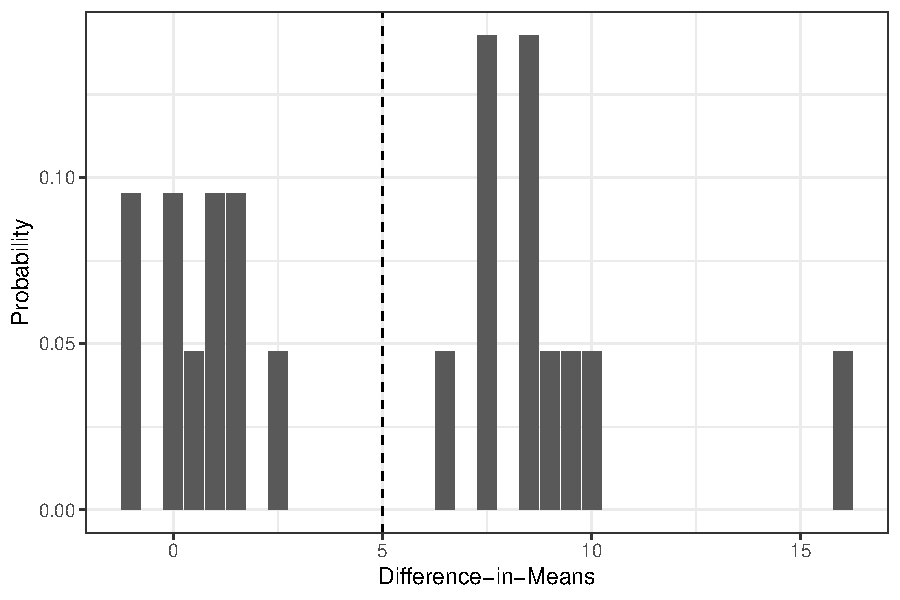
\includegraphics[width=\linewidth]{cra_est_dist_plot.pdf}
\caption{Difference-in-Means estimator in ``Village heads'' example}
\end{figure}
\end{itemize}
\end{frame}
%------------------------------------------------------------------------
\begin{frame}
\frametitle{Next steps}
\vfill
\begin{itemize} \vfill
\item What happens when the size of our experiment grows large? \vfill
\item Consistency of Difference-in-Means estimator for ATE \vfill
\item Asymptotic validity of hypothesis tests about ATE \vfill
\end{itemize} \vfill
\vfill
\end{frame}
%------------------------------------------------------------------------

\end{document}